% leben.tex
\documentclass[dvisvgm]{standalone}

\usepackage{amsmath}
\usepackage[usenames,dvipsnames]{xcolor}
\usepackage{tikz}
\usetikzlibrary {arrows.meta,
                 calc,
                 decorations.pathreplacing,
                 positioning,
                 shapes.geometric}

 \tikzset{
        base/.style={draw, align=center, minimum height=4ex},
        proc/.style={base, rectangle, text width=8em},
        io/.style={trapezium, trapezium left angle=70, trapezium right
                   angle=110, draw, text width=8em, %minimum width=2cm, 
                   %minimum height=1cm
                   },
        test/.style={base, diamond, aspect=2,
                     %text width=5em
                     },
        term/.style={proc, rounded corners},
        myarrow/.style={-Stealth, line width=0.25mm},
 }

\begin{document}

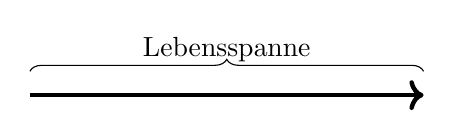
\begin{tikzpicture}
    \draw[->, ultra thick] (0,0) -- (5,0);
    \draw[decorate, decoration={brace, raise=2ex, amplitude=1ex}] 
         (0,0) -- (5,0) node[midway, above=2ex]{Lebensspanne};
\end{tikzpicture}

\end{document}
